\chapter{Analyse des données}

TODO : décrire vite fait chaque table ? \\
TODO : raconter ce qu'on a découvert dans les données et comment (sans requêtes SQL) -> les données ne sont pas bonnes, nous les avons vérifiées, grâce à des requêtes (vérifications internes) et à d'autres sources externes (wikipédia...) \\
 - les causes de morts qui s'imbriquent \\
 - la somme de niveau 1 différentes de celles de niveau 2 \\
 - les données des années 79 - 80 sont des estimations (chiffres ronds) car absence de données pour ces années là \\
 - pour les néoplasies, les causes renseignées pour la mort sont les causes les plus précises (plus d'imbrications des causes et donc de doublons des morts) \\
 ...

 Les données fournies contiennent des informations sur les causes de décès et la population en Angleterre et au Pays de Galles entre 1979 et 1992, sous la forme de tables. Nous allons tout d'abord analyser ces tables, afin d'en comprendre le contenu et d'en vérifier la validité. \\

\begin{paragraph}
Les données sont formées de 19 tables, liées entre elles par des clés étrangères. Nous avons tout d'abord remarqué que les données des deux premières années (79 et 80) sont des estimations (chiffres ronds et calculs justes). En effet, les données étaient manquantes pour ces deux années, et elles ont été estimées par rapport aux évolutions des autres années. Commençons tout d'abord par les tables concernant la population. La table principale est "7992pops", et compte 214 396 lignes. Elle contient le nombre de personnes vivantes, dans les régions citées précédemment, en fonction de l'année, du district, de l'age et du sexe. Ces différentes informations (sauf l'année) sont en fait des identifiants, à mettre en relation avec d'autre tables. Nous avons vérifier, grâce à une requête SQL, que la clé de cette table était bien composé des identifiants de county, district, sexage et de l'année.\\
Les identifiants de county et de district peuvent donner le nom du district concerné, dans la table "cdlist". Il existe 403 districts, contenus dans des county, eux-même contenus dans des régions. \\
Ils permettent aussi de faire le lien avec la table "areaclas", qui contient elle aussi pour chaque paire d'identifiants le nom du district, ainsi que les codes et noms des familles, groupes et clusters. Ceux-ci sont des classifications des districts selon des critères économiques. \\
A partir de l'identifiant du county, on peut retrouver son nom et l'identifiant de la région à laquelle il appartient grâce à la table "county". Il existe 54 county.\\
De la même façon, à partir de l'identifiant de la région, on peut faire le lien avec la table "region", qui permet de retrouver son nom (il y en a 11 en tout). \\
On peut ensuite retrouver l'âge et le sexe de la catégorie à partir de l'identifiant sexage, que l'on retrouve dans la table "sexage". Cette table contient les identifiants associés à des labels, ceux-ci étant de la forme M1-4 ou encore W5-9, représentant respectivement des garçons agés de 1 à 4 ans, et des filles agées de 5 à 9 ans. Ce découpage permet de classer la population selon 38 catégories de sexage.\\
\end{paragraph}

\begin{paragraph}
Nous allons maintenant nous intéresser aux données concernant les morts. Ces données étant vraiment très imposantes, elles sont séparées en 11 tables, une par région : "yorkhumb", "westmids", "stheast", "wales", "sthwest", "nthwest", "london", "ntheast", mersey", "eastmids" et "eastern". De même que précédement, les différentes lignes correspondent au nombre de morts selon l'année, le disctrict, la catégorie sexage, avec en plus la cause. \\
La cause est en fait un identifiant correspondant à une ligne de la table "causes". Chaque cause a un nom, un niveau et un père. Elles sont réparties selon un arbre de causes : la cause 1 correspond à la cause "toutes les causes", cette cause a des fils qui elles-mêmes ont des fils, et plus le niveau est élevé, plus la cause de mort est précise. Le père de la cause correspond donc à son père dans l'arbre. Normalement, toutes les morts de causes de niveau 1 devraient être égales à toutes les morts de cause de niveau 2 ainsi que toutes les sommes sur les niveau. En réalité, grâce des requêtes SQL adéquates, nous avons réalisé que les sommes n'étaient pas égales. Ceci est probablement du à des erreurs ou des oublis lors du remplissage des certificats. \\
\end{paragraph}

\pagebreak


\chapter{Modélisation de l'entrepôt et des cubes}

\section{Hypercube Population}
\begin{figure}[h!]
    \centering
    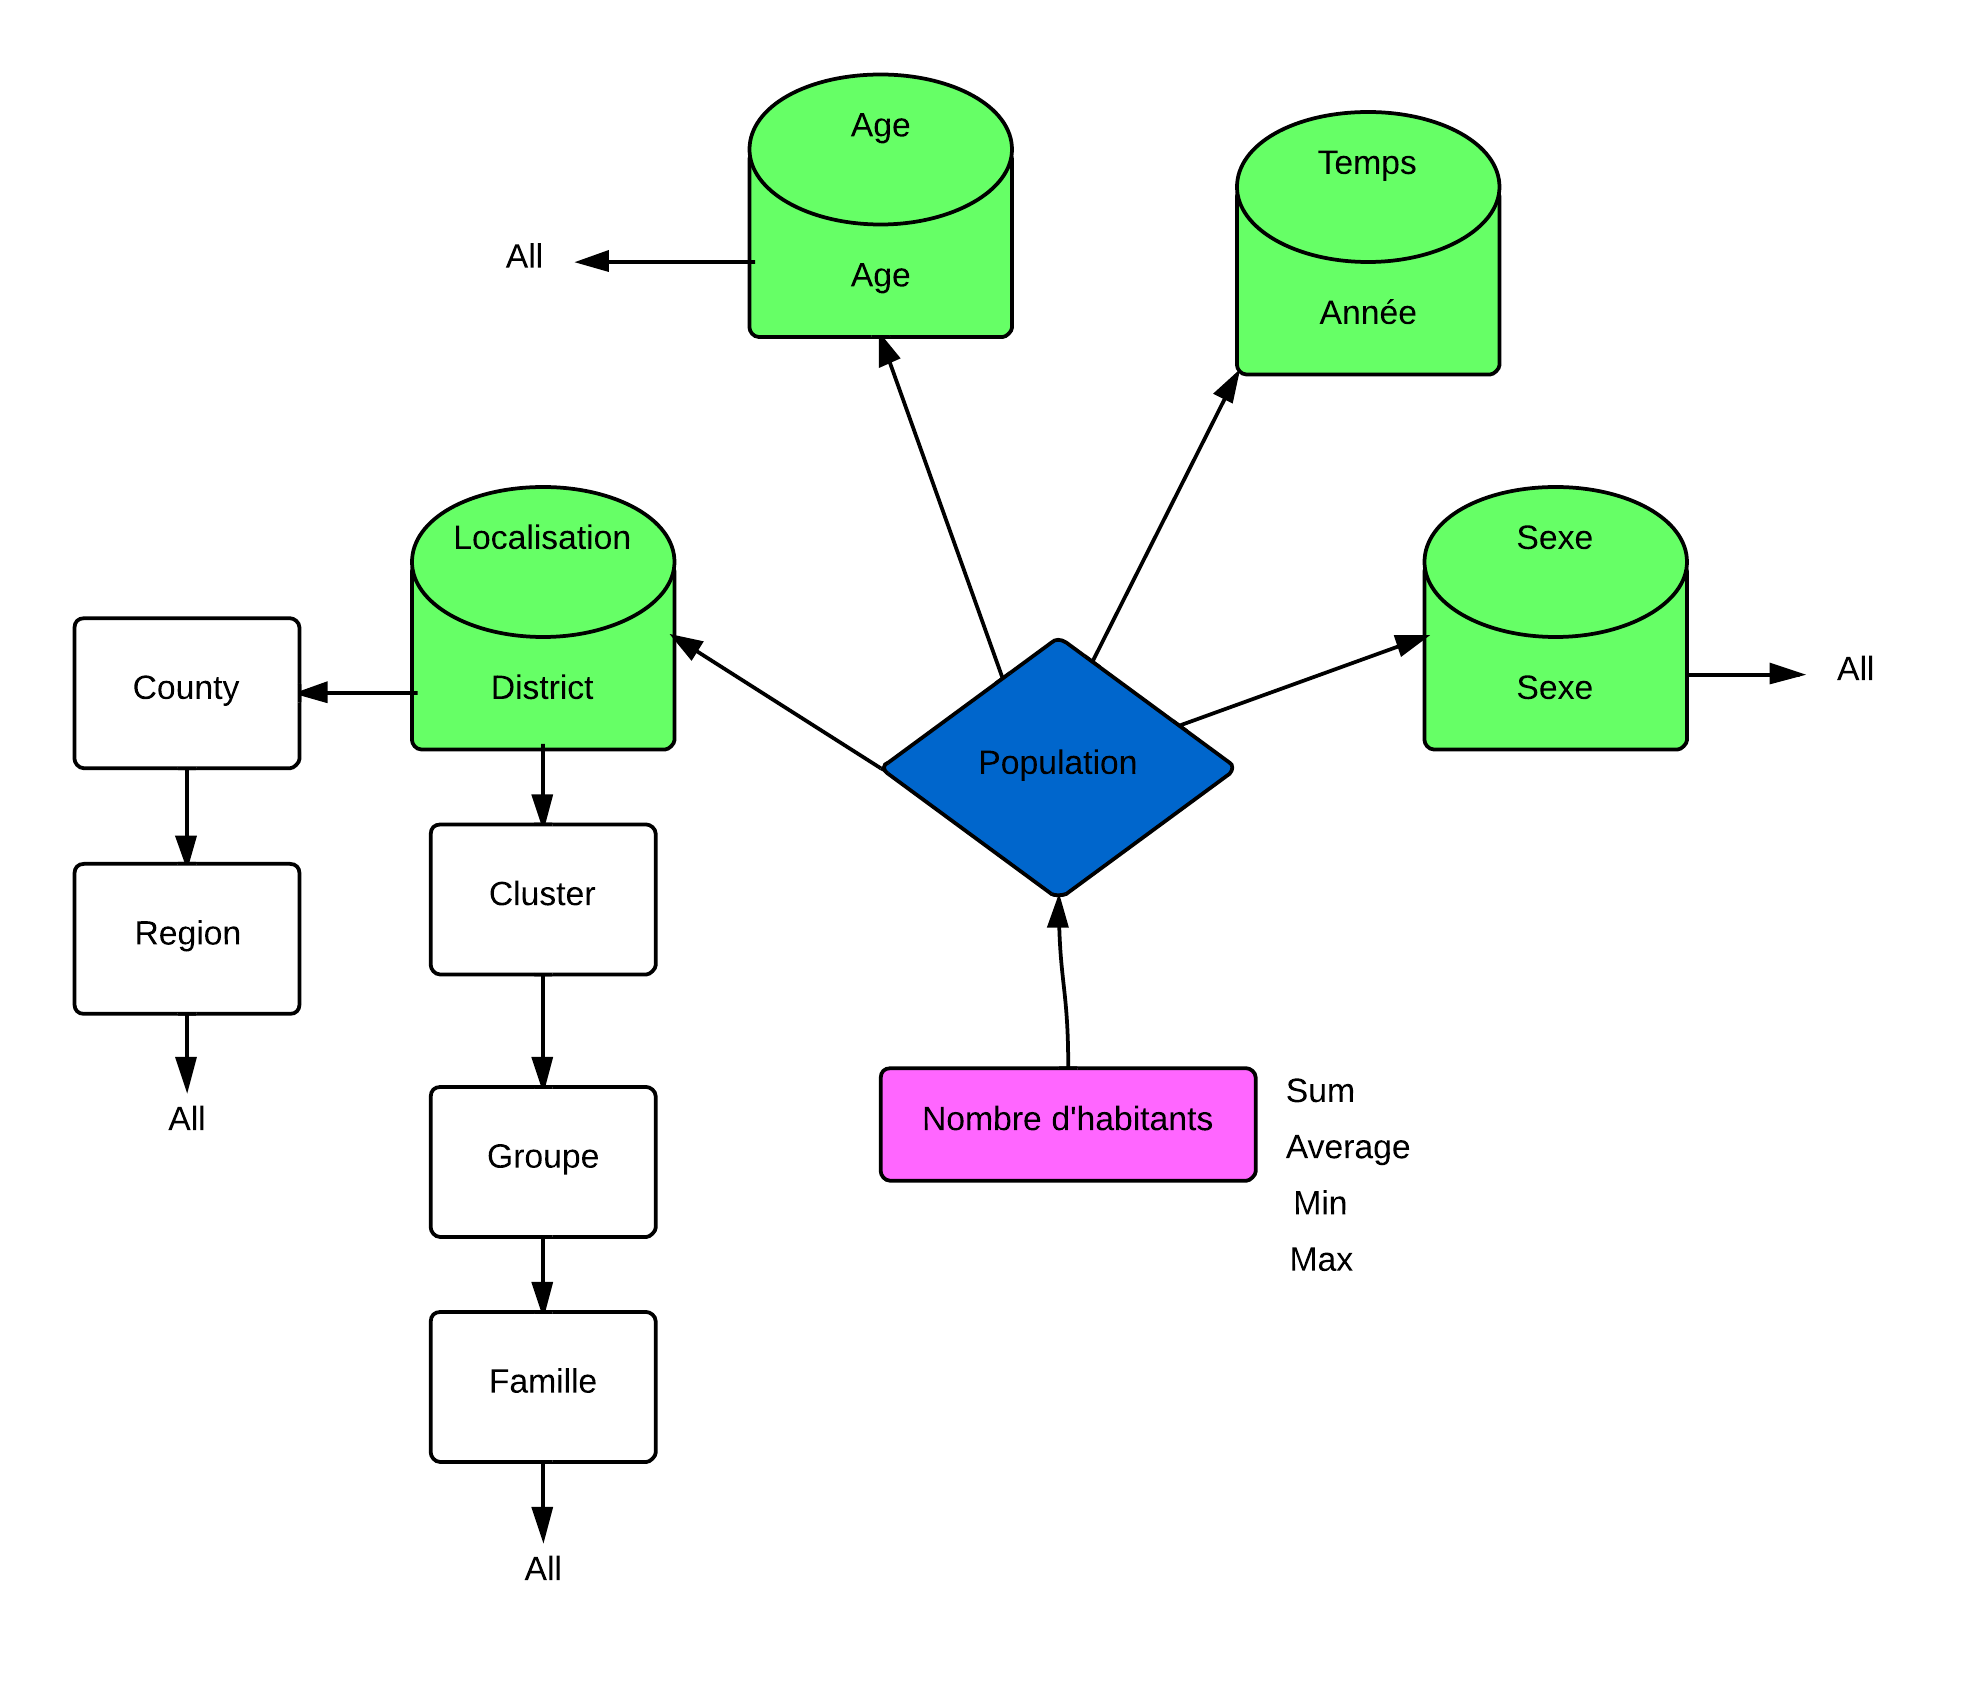
\includegraphics[width=\linewidth]{images/pop/cube.png}
    \caption{Modèle conceptuel de l'hypercube Population}
    \label{conception_cube_pop}
\end{figure}

\section{Hypercube Nombre de morts}
\begin{figure}[h!]
    \centering
    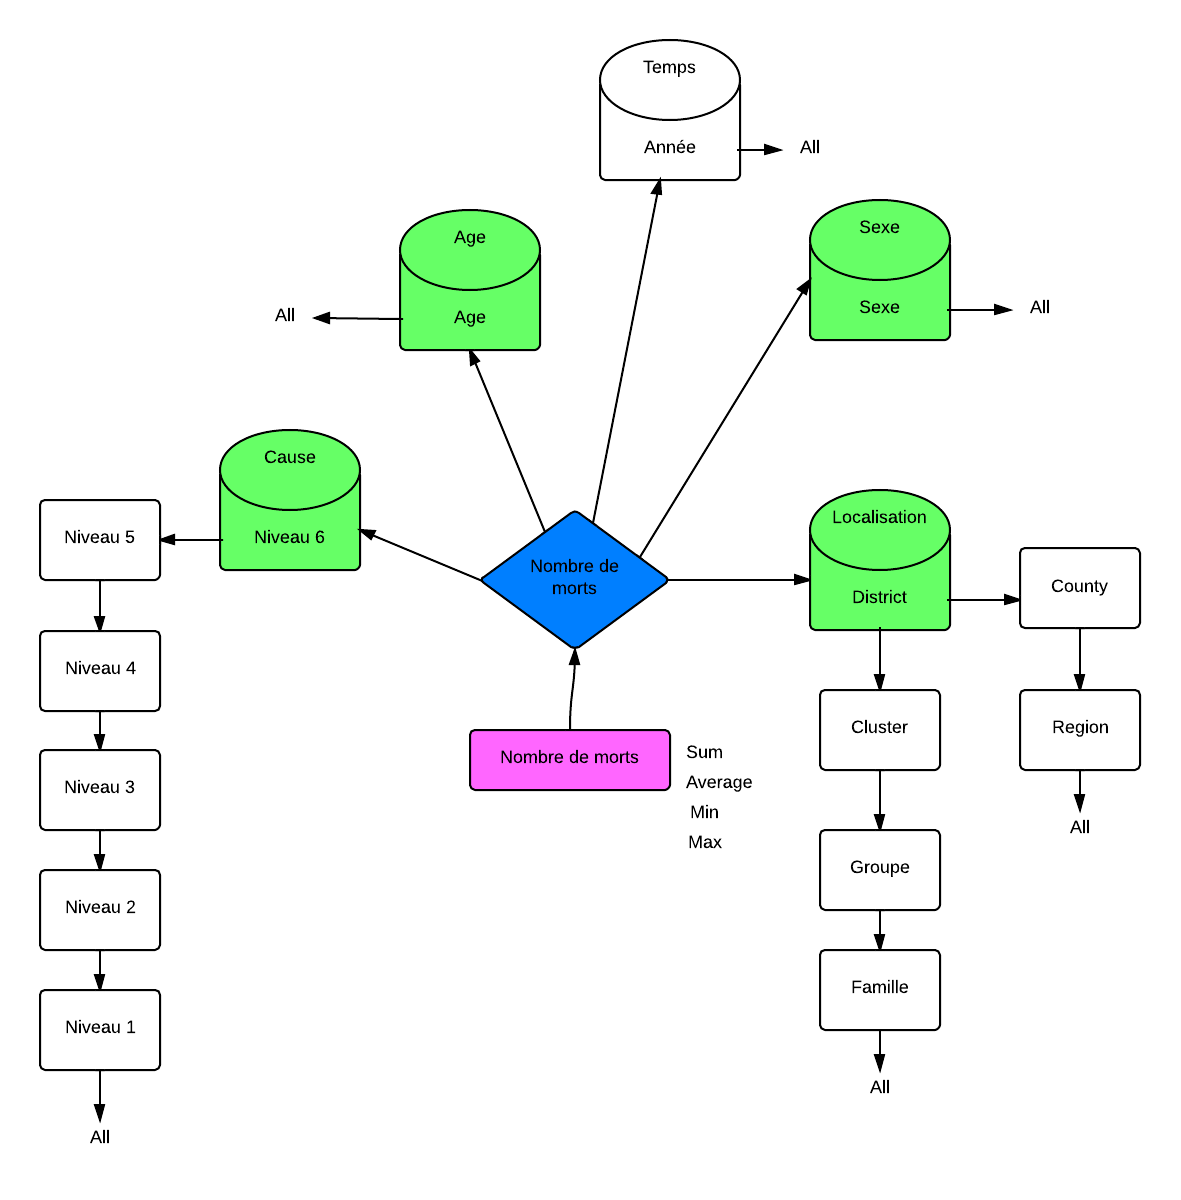
\includegraphics[width=\linewidth]{images/cubeNbMorts.png}
    \caption{Modèle conceptuel de l'hypercube Nombre de morts}
    \label{conception_cube_nombre_morts}
\end{figure}

\section{Hypercube Néoplasies}
\begin{figure}[h!]
    \centering
    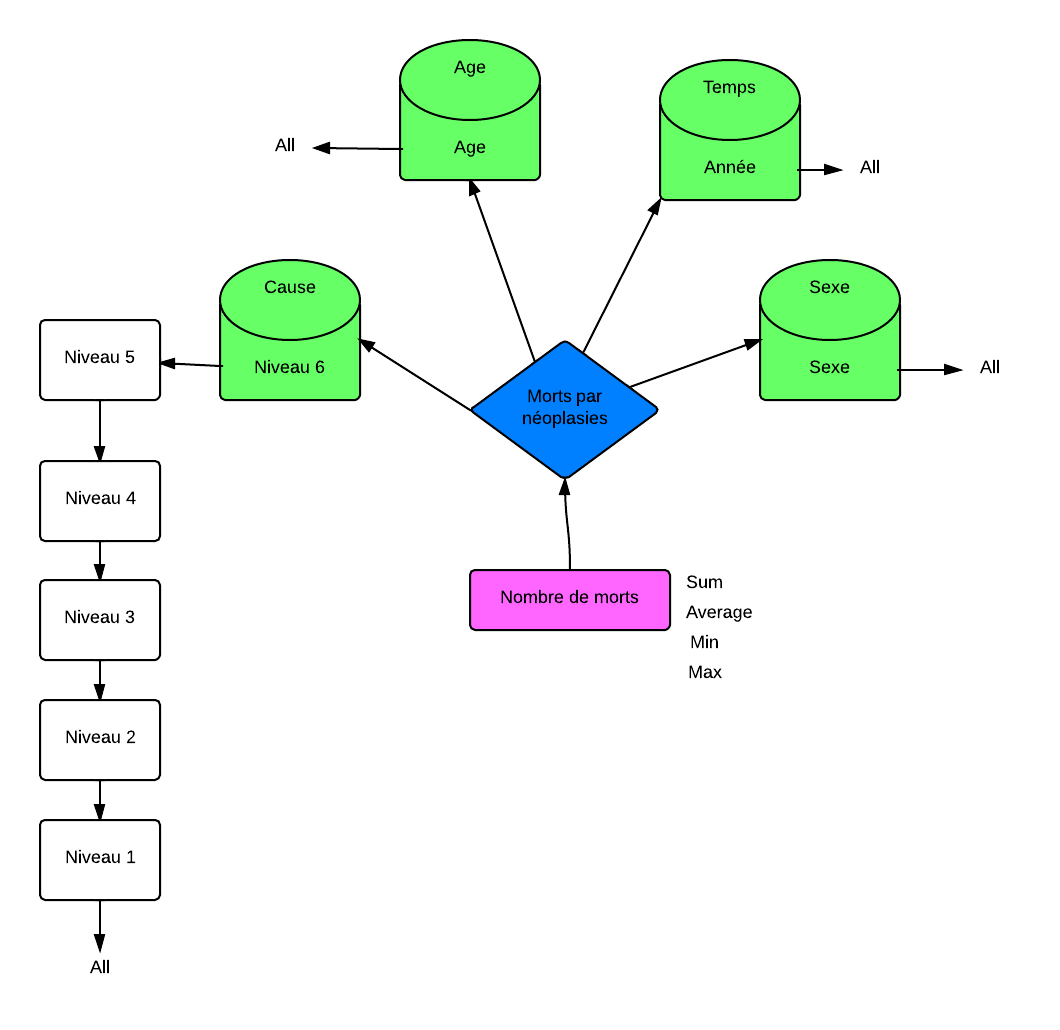
\includegraphics[width=\linewidth]{images/cubeNeo.png}
    \caption{Modèle conceptuel de l'hypercube Néoplasies}
    \label{conception_cube_néoplasies}
\end{figure}

\section{Entrepôt}
\begin{figure}[h!]
    \centering
    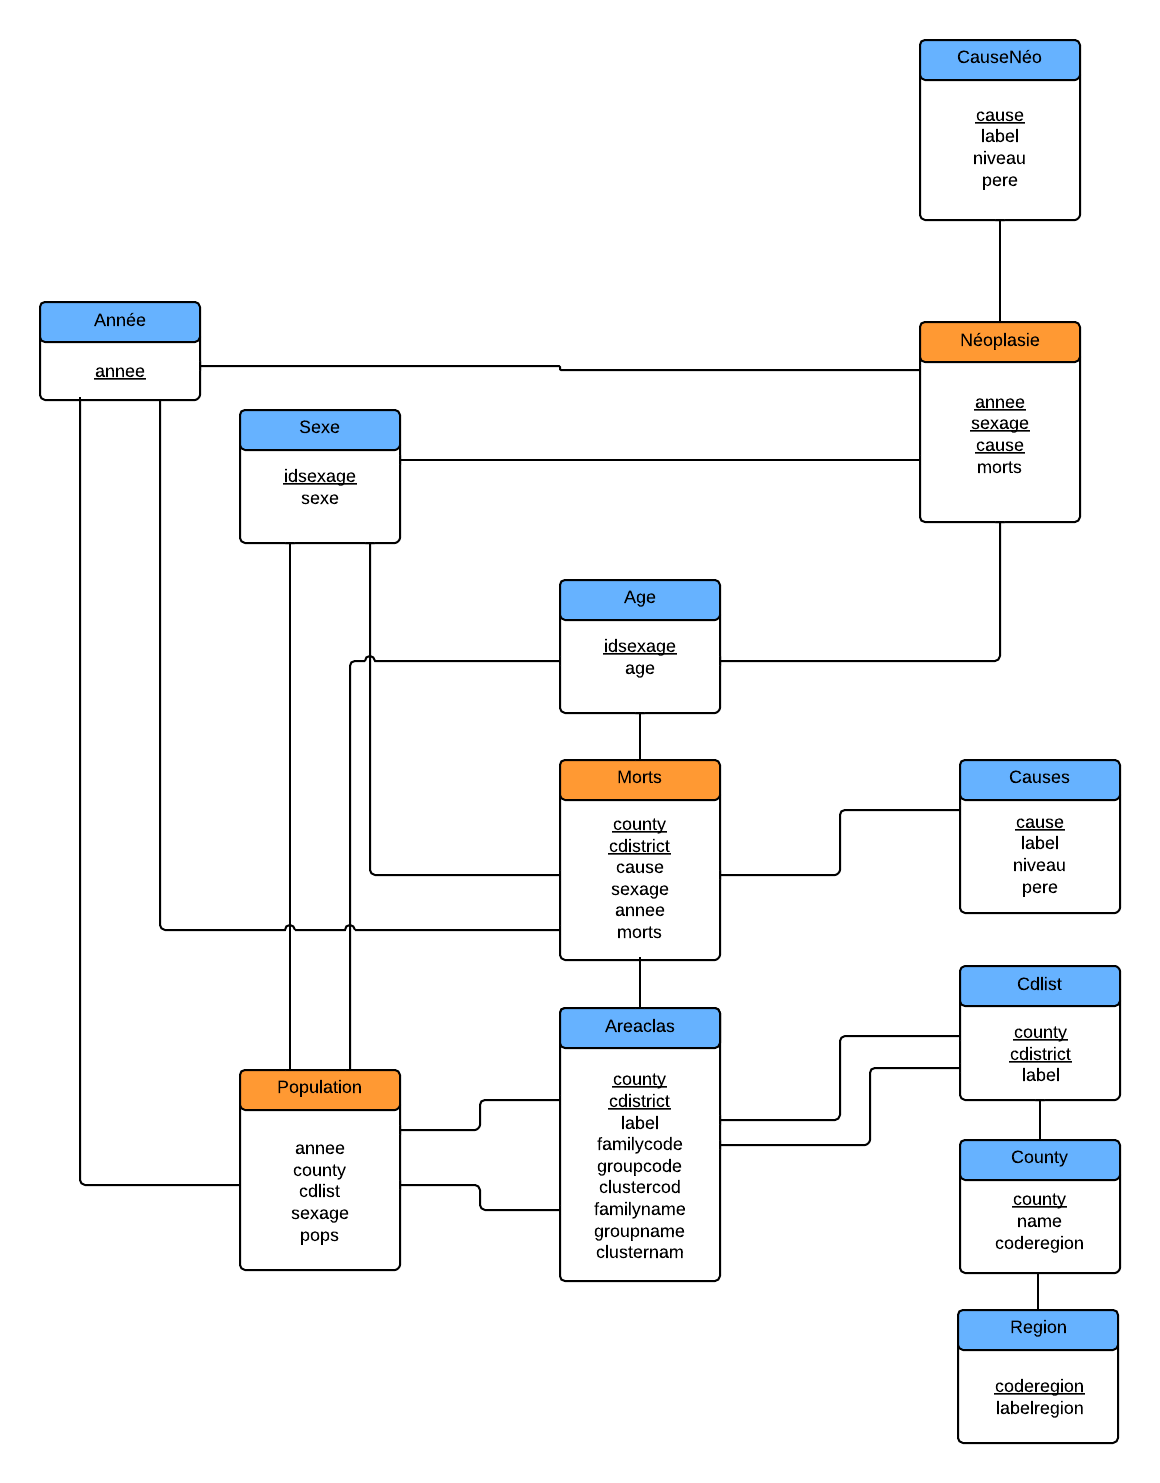
\includegraphics[width=\linewidth]{images/entrepot.png}
    \caption{Modèle logique de l'entrepôt}
    \label{conception_cube_néoplasies}
\end{figure}


\pagebreak


\chapter{Transformations des tables d'origine}

TODO : enlever les requetes SQL, reformuler pour avoir pour chaque transfo : les sources, la destination et les opérations effectuées) et completer les transformations réalisées pour tous les cubes

\section{Séparation des données de sexe et d'age}

    Vu le format des données de la table SexAge, dissocier l'effet du sexe et de l'âge s'avérait hardu.

    Nous avons donc modifié la table en créant deux nouvelles colonnes: Sex, nvarchar qui contiendra le sexe (M/F), et Age,
    nvarchar qui contiendra la tranche d'âge (<1, 10-14, ...).

    Nous avons alors lancé la requête suivante afin de séparer les données de ``sexage'' sur ces deux colonnes :

    \begin{lstlisting}[frame=single, language=SQL]
UPDATE sexage
SET Sex=LEFT(label, 1), Age=RIGHT(label, LEN(label) - 1);
    \end{lstlisting}

\section{Table temporelle}

    Requête pour initialiser la table \textit{year} après sa création (une colonne de type entier et clé primaire)

    \begin{lstlisting}[frame=single, language=SQL]
INSERT INTO Annee
SELECT     [YEAR]
FROM [7992pops]
GROUP BY [YEAR]
ORDER BY [YEAR]
    \end{lstlisting}

\section{Visualisation des données}

    Nous avons exploré les données mises à notre disposition, en essayant de trouver des motifs, incohérences et autres motifs particuliers
    dans ces dernières.

    Pour cela, nous avons effectué plusieurs requêtes SQL, comme cette requête qui donne la répartition des décès par sexe pour chaque
    cause.

    \begin{lstlisting}[frame=single, language=SQL]
SELECT sexage.SEX, causes.LABEL, COUNT(*) AS Number
FROM london INNER JOIN
    sexage ON london.SEXAGE = sexage.SEXAGE INNER JOIN
    causes on london.CAUSE = causes.CAUSE
GROUP BY sexage.sex, causes.label
    \end{lstlisting}

    On a donc découvert que, surprise !, il n'y a pas de décès ayant pour cause un avortement, chez le sexe masculin.

\section{Incohérences dans les nombre de morts}

    En analysant la table des morts de chaque région, nous avons remarqué que la somme des morts par cause de niveau 2 était
    inférieure au nombre de morts par cause de niveau 1 (càd de toutes les causes de mort).

    Si ceci est dû en partie à des certificats de décès qui ne sont pas correctement remplis, il existe aussi une autre cause,
    renseignée dans le document fourni (\textbf{``local mortaility datapack.pdf''})~: Un nouveau certificat pour les morts néonatales
    a été introduit en 1986, et ces morts ne sont plus rentrées sous la cause ``Certain conditions originating in the perinatal
    period'' depuis cette date là.

    On peut voir cette différence dans le nombre de morts de la table ``westmids'' (par exemple) avec la requête suivante :

    \begin{lstlisting}[frame=single, language=SQL]
SELECT causes.NIVEAU, SUM(westmids.DEATHS) AS TotalDeaths
FROM westmids INNER JOIN causes ON westmids.CAUSE = causes.CAUSE
GROUP BY causes.NIVEAU
HAVING (causes.NIVEAU = 1) OR (causes.NIVEAU = 2)
    \end{lstlisting}

    La solution qu'on a choisie est de rajouter une nouvelle cause de mort de niveau 2 représentant une cause indéfinie, afin
    de ne pas sous-estimer le nombre de morts en ignorant ceux dont la cause de niveau 2 n'est pas renseignée.

    La requête utilisée pour réaliser cette opération est détaillée plus bas, dans la partie exploitation de données.

\section{Union des données dans une nouvelle table}

    Afin d'exploiter ces données, nous avons créée deux nouvelles tables centralisant toutes les morts des différentes régions.

    Selon l'utilisation désirée (étude des causes de niveau 2, étude de la néoplasie), des conditions sont posées afin
    de minimiser le volume des données manipulées.

    Par exemple, pour l'étude des causes de niveau 2.

    \begin{lstlisting}[frame=single, language=SQL]
INSERT INTO deaths
SELECT *
FROM
(
    SELECT london.* FROM london INNER JOIN causes ON london.cause = causes.cause WHERE causes.niveau <= 2 UNION
    SELECT eastmids.* FROM eastmids INNER JOIN causes ON eastmids.cause = causes.cause WHERE causes.niveau <= 2 UNION
    ...
)
    \end{lstlisting}


\section{Exploitation des nouvelles données}

    Afin d'exploiter ces données, nous avons créée deux nouvelles tables centralisant toutes les morts des différentes régions.

    \begin{lstlisting}[frame=single, language=SQL]
SELECT deaths.*
FROM deaths INNER JOIN causes
        ON deaths.cause = causes.cause
WHERE causes.niveau <= 2
    \end{lstlisting}

    Et comme vu précédemment, il existe un gap entre le nombre total de morts si on regarde les causes de niveau 2 ou le nombre
    total de morts (cause de niveau 1).

    \begin{lstlisting}[frame=single, language=SQL]
SELECT causes.niveau, SUM(deaths.deaths)
FROM deaths INNER JOIN causes
        ON deaths.cause = causes.cause
    \end{lstlisting}

    Afin de corriger cette incohérence, nous rajoutons comme prévu une cause de niveau 2 représentant une cause non renseignée
    et lui donnons l'id \textit{120}.

    Nous exécutons alors cette requête qui va calculer le gap entre les morts de niveau 1 et de niveau 2, puis rajouter une ligne
    s'il y a des morts non renseignées (avec la cause que l'on vient de créer).

    \begin{lstlisting}[frame=single, language=SQL]
INSERT INTO deaths
SELECT h.year, h.county, h.cdistrict, 120, h.sexage, h.delta
FROM (
    SELECT t.year, t.county, t.cdistrict, t.sexage,
    (
        (
            SELECT sum(tt1.deaths)
            FROM deaths AS tt1, causes AS cc1
            WHERE tt1.cause = cc1.cause
            AND cc1.niveau = 1
            AND tt1.year = t.year
            AND tt1.county = t.county
            AND tt1.cdistrict = t.cdistrict
            AND tt1.sexage = t.sexage
        )
        -
        (
            SELECT sum(tt2.deaths)
            FROM deaths AS tt2, causes AS cc2
            WHERE tt2.cause = cc2.cause
            AND cc2.niveau = 2
            AND tt2.year = t.year
            AND tt2.county = t.county
            AND tt2.cdistrict = t.cdistrict
            AND tt2.sexage = t.sexage
        )
    ) AS delta
    FROM deaths AS t
    GROUP BY t.year, t.county, t.cdistrict, t.sexage
) AS h
WHERE h.delta > 0
    \end{lstlisting}

\pagebreak

\chapter{Indicateurs et validation}

TODO : trouver pour chaque cube des indicateurs et les utiliser pour montrer qu'on a validé nos données (c'est-à-dire que les données étaient toujours les mêmes avant et après nos modifications de tables)

\section{Population}
Les validations suivantes ont été appliquées sur le cube Population afin de valider l'intégrité des données de celui-ci. Les résultats obtenus lors de l'exploration du cube ont été recoupées avec les données des tables par les requêtes SQL adéquates :
\begin{itemize}
    \item Population totale en 1992 : 51 276 887
    \item Population totale en 1992 dans le 1er county : 6 904 554
    \item Population totale en 1992, de sexe masculin et d'âge inférieur à un an : 355 930
    \item Population totale en 1992, de sexe masculin et d'âge inférieur à un an dans le 1er district et le 1er county du cluster Central London : 18
\end{itemize}


\pagebreak
